\documentclass{noithesis}

\newtheorem{theorem}{定理}[section]
\newtheorem{definition}[theorem]{定义}
\newtheorem{lemma}[theorem]{引理}
\newtheorem{property}{性质}[theorem]


\begin{document}
	
	\title{2023 程序设计 II 荣誉课程大作业报告}
	\author{中国人民大学~~李修羽}
	
	\maketitle
	
	\begin{abstract}
		本文主要探究了基于 Qt 图形界面应用设计的不围棋联网对战软件制作过程,对一些重要功能的实现进行了说明,同时对于团队分工过程有一定记录。在联网体系之外,额外探究了不围棋 AI 的算法设计与实现。
	\end{abstract}

	\tableofcontents
	\setcounter{page}{0}
	\thispagestyle{empty}
	\newpage
	
	\section{团队构成}
	
	\subsection{闲话}
	
	理论上这个大作业一个人也可以做,但是既然都称之为团队大作业了,那就团队做。
	
	\subsection{小组分工}
	
	笔者负责了项目 UI 的主要设计、棋盘逻辑的编写和报告的撰写。
	
	冯友和同学负责了项目框架的建构、初始 bot 的设计。
	
	赵培宇同学负责了棋盘的生成、按钮的部分实现。
	
	\section{Qt 图形界面应用设计}
	
	
	\subsection{UI 设计}
	
	\begin{figure}[!htb]{
		\centering
		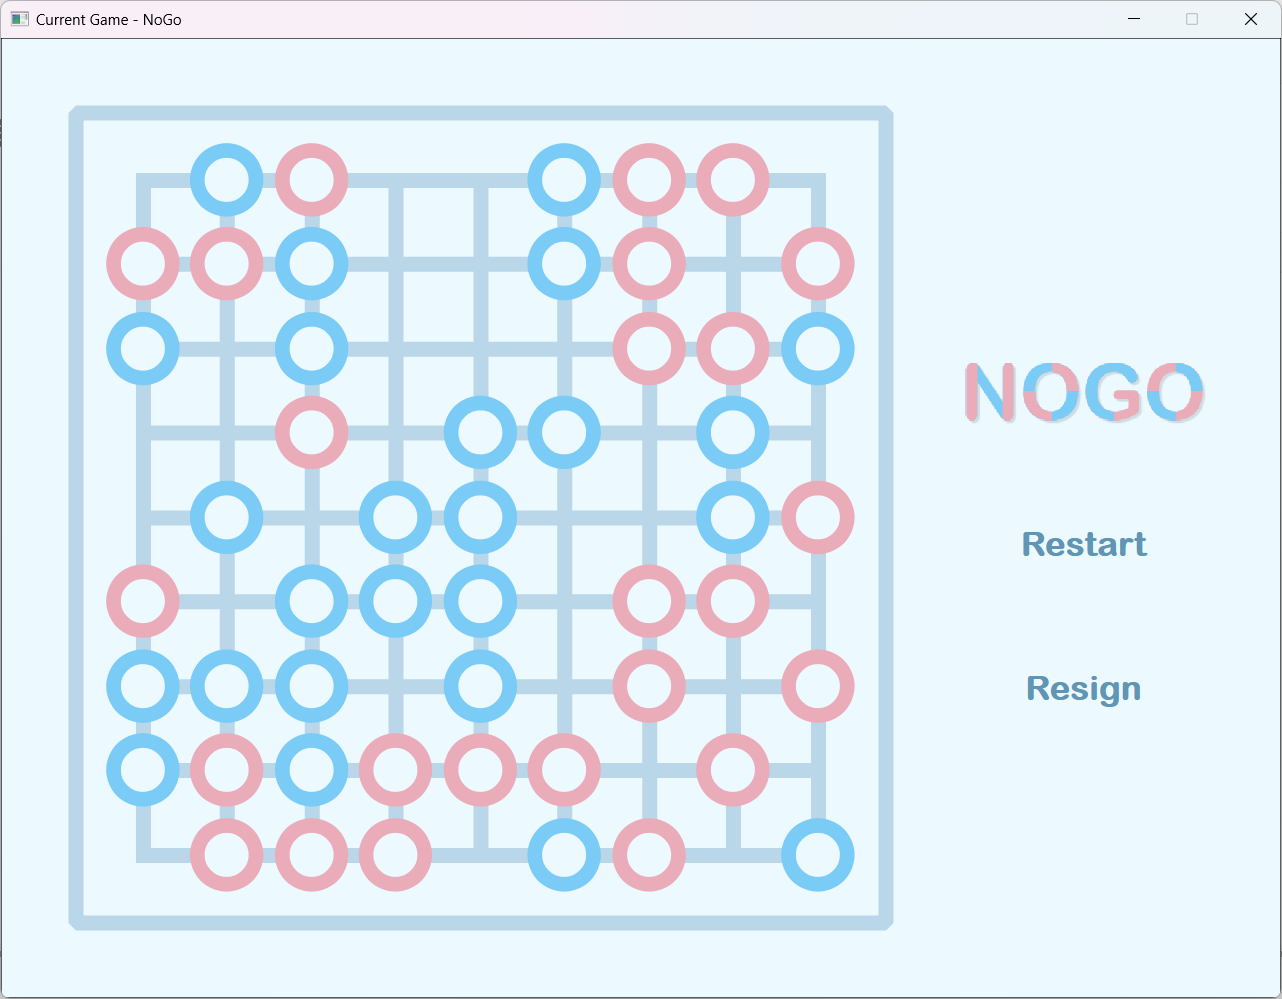
\includegraphics[width=0.8\textwidth]{img/UI.png}
		\counterwithin{figure}{subsection}
		\caption{demo 示例}
	}
	\end{figure}

	本应用 UI 设计\footnote{部分设计参考:https://github.com/epcm/QtNoGo}采用扁平化的设计风格,搭配上饱满、明亮、可爱且前卫的颜色设计,亮度统一且冷暖色调搭配,具有舒适的观感。字体使用 Sans-serif 字体 Arial Rounded MT Bold,平衡现代感和亲和感。棋子中心保留背景色,使棋盘整体更为协调。
	
	由于棋盘大小可以自定义,棋盘采用程序绘图而非图片覆盖的形式,可以根据棋盘的大小自适应调整棋盘线条粗细和棋子大小,保持程序页面分辨率相对不变。
	
	\begin{figure}[!htb]{
			\centering
			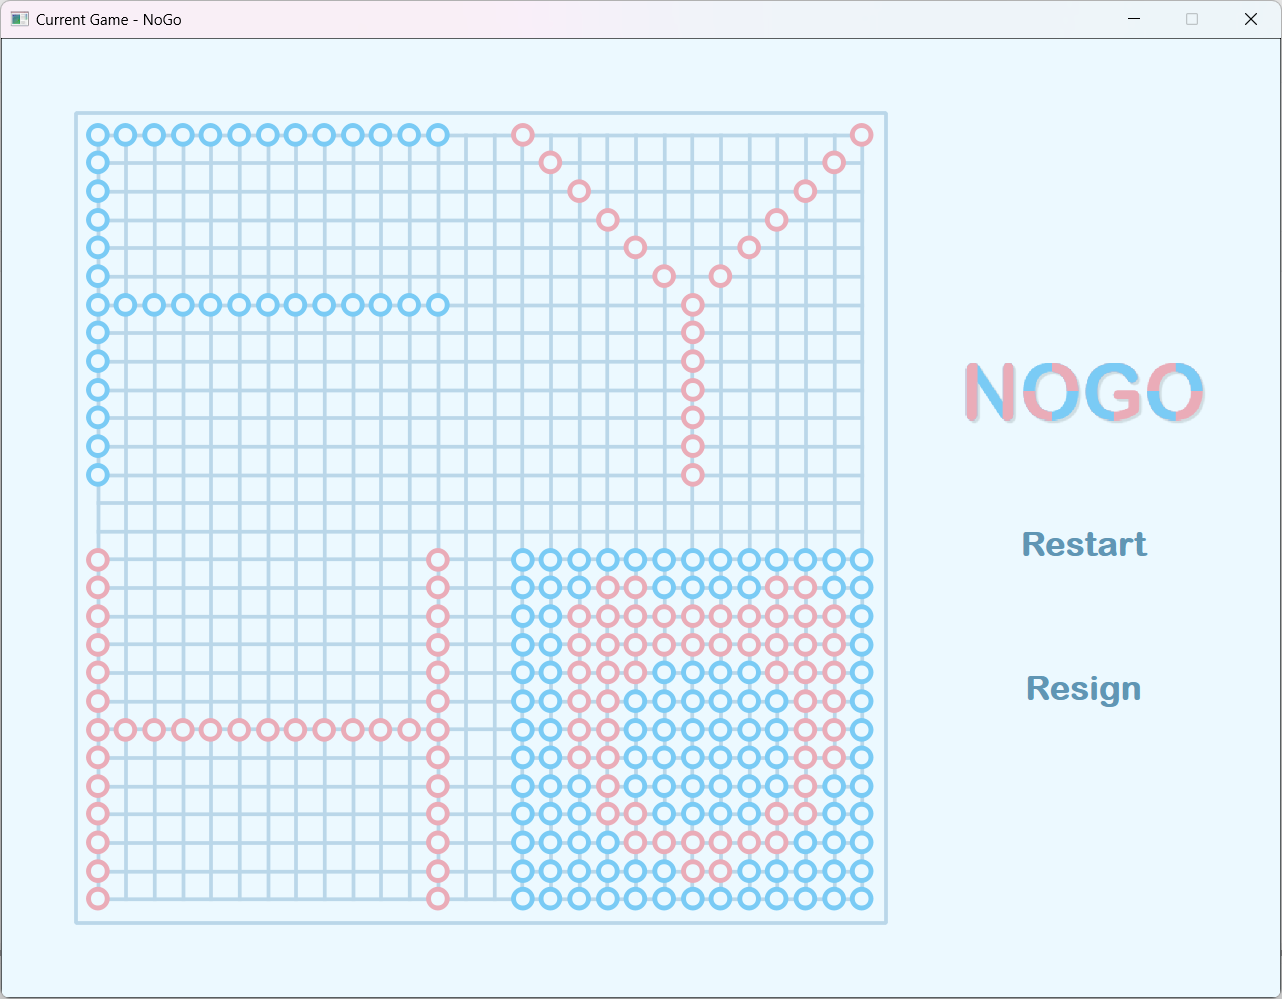
\includegraphics[width=0.8\textwidth]{img/fyh.png}
			\counterwithin{figure}{subsection}
			\caption{自定义棋盘大小~(29)}
		}
	\end{figure}
	
	Logo 以棋子底色为设计基础,增加了颜色块的分割,具有棋类游戏的风格,也维持了项目的主要设计基调。

	\subsection{基本逻辑}
	
	\begin{verbatim}
	|-- Qt-NoGo
	    |-- mynogo.pro            // QMake 项目管理文件
	    |-- mynogo.pro.user
	    |-- Headers
	    |   |-- bot.h
	    |   |-- gamewidget.h      // 控制程序运行的类
	    |   |-- judge.h           // 控制棋盘操作和逻辑的类
	    |   |-- mainwindow.h
	    |   |-- messagebox.h
	    |   |-- startwidget.h
	    |-- Sources
	    |   |-- bot.cpp           // 随机下棋 bot
	    |   |-- gamewidget.cpp
	    |   |-- judge.cpp
	    |   |-- main.cpp          // 程序入口
	    |   |-- mainwindow.cpp
	    |   |-- messagebox.cpp
	    |   |-- startwidget.cpp
	    |-- Forms
	    |   |-- gamewidget.ui
	    |   |-- mainwindow.ui
	    |   |-- startwidget.ui
	    |-- Resources
	    |   |-- img.qrc           // 图片配置文件
	    |-- img
	    |   |-- logo.png          // Logo 图片
	    |-- report                // 项目报告
	    |-- README.md
	\end{verbatim}

	基本逻辑为 main 打开 mainwindow,mainwindow 切换到 startwidget 和 gamewidget,由 gamewidget 初始化 judge 开始游戏。

	\subsection{棋盘逻辑和结局判断}
	
	由于最后 NoGo-Cup 给 AI 的限时是 1s,留给 AI 计算的时间并不充裕,所以本项目采用了高效率的棋盘底层逻辑,以期为 AI 的运行提供尽可能多的时间。
	
	相较于传统的 dfs 判断棋子,笔者创新性地采用了启发式合并的方法来判断棋子的连通性与气数,在 judge.h 中的定义如下:
	
	\begin{lstlisting}
	typedef std::pair<int, int> Item;
	typedef std::vector<Item> ItemVector;
	typedef std::set<Item> LibertySet;

	int board[CHESSBOARD_SIZE + 2][CHESSBOARD_SIZE + 2]; // 当前棋盘状态
	int chessBelong[CHESSBOARD_SIZE + 2][CHESSBOARD_SIZE + 2]; // 棋子属于的棋子块
	int blockVis[(CHESSBOARD_SIZE + 2) * (CHESSBOARD_SIZE + 2)]; // 棋子块至多只能累加一次
	int blockCnt; // 棋子块个数
	
	LibertySet blockLiberty[(CHESSBOARD_SIZE + 2) * (CHESSBOARD_SIZE + 2)]; // 气的 Set
	ItemVector chessBlock[(CHESSBOARD_SIZE + 2) * (CHESSBOARD_SIZE + 2)]; // 棋子块的编号
	std::vector<int>mergedBlock;
	\end{lstlisting}

	本程序用 vector 存储每一个连通块棋子的位置,用 set 存储每一个连通块气的位置。对于一次合并,将两端连通块的 vector 和 set 分别启发式合并即可。此处采用 set 是因为其本身具有判重的特性,可以在合并时对气做出高效率的处理。
	
	\begin{lstlisting}
		
	void Judge::MergeSet(LibertySet &x, LibertySet y)
	{
		if(x.size() < y.size()) std::swap(x, y);
		for(Item u : y) x.insert(u);
	}
	void Judge::MergeBlock(int x, int y) // 启发式合并
	{
		if(chessBlock[x].size() < chessBlock[y].size()) std::swap(x, y);
		MergeSet(blockLiberty[x], blockLiberty[y]);
		for(Item u : chessBlock[y])
		{
			chessBlock[x].push_back(u);
			chessBelong[u.first][u.second] = x;
		} // 合并
		chessBlock[y].clear(); // 清空
	}
	\end{lstlisting}

	相较于 dfs 判断单次 $O\left(n^2\right)$ 的复杂度,启发式合并的复杂度可以做到 $O\left(\log^2 n\right)$,且此处的 $n^2$ 仅为理论上界,对于大规模棋盘(例如 $20\times 20$)有极高的效率。
	
	对于一次落子操作,如果落子后判负,会弹出此处无法落子的弹窗。同时在一次操作超时后,会直接超时判负。对于现有版本来说,页面实现了认输按钮,玩家在无法落子后可以等到超时判负,也可以认输判负。
	
	\begin{figure}[htbp]
		\centering
		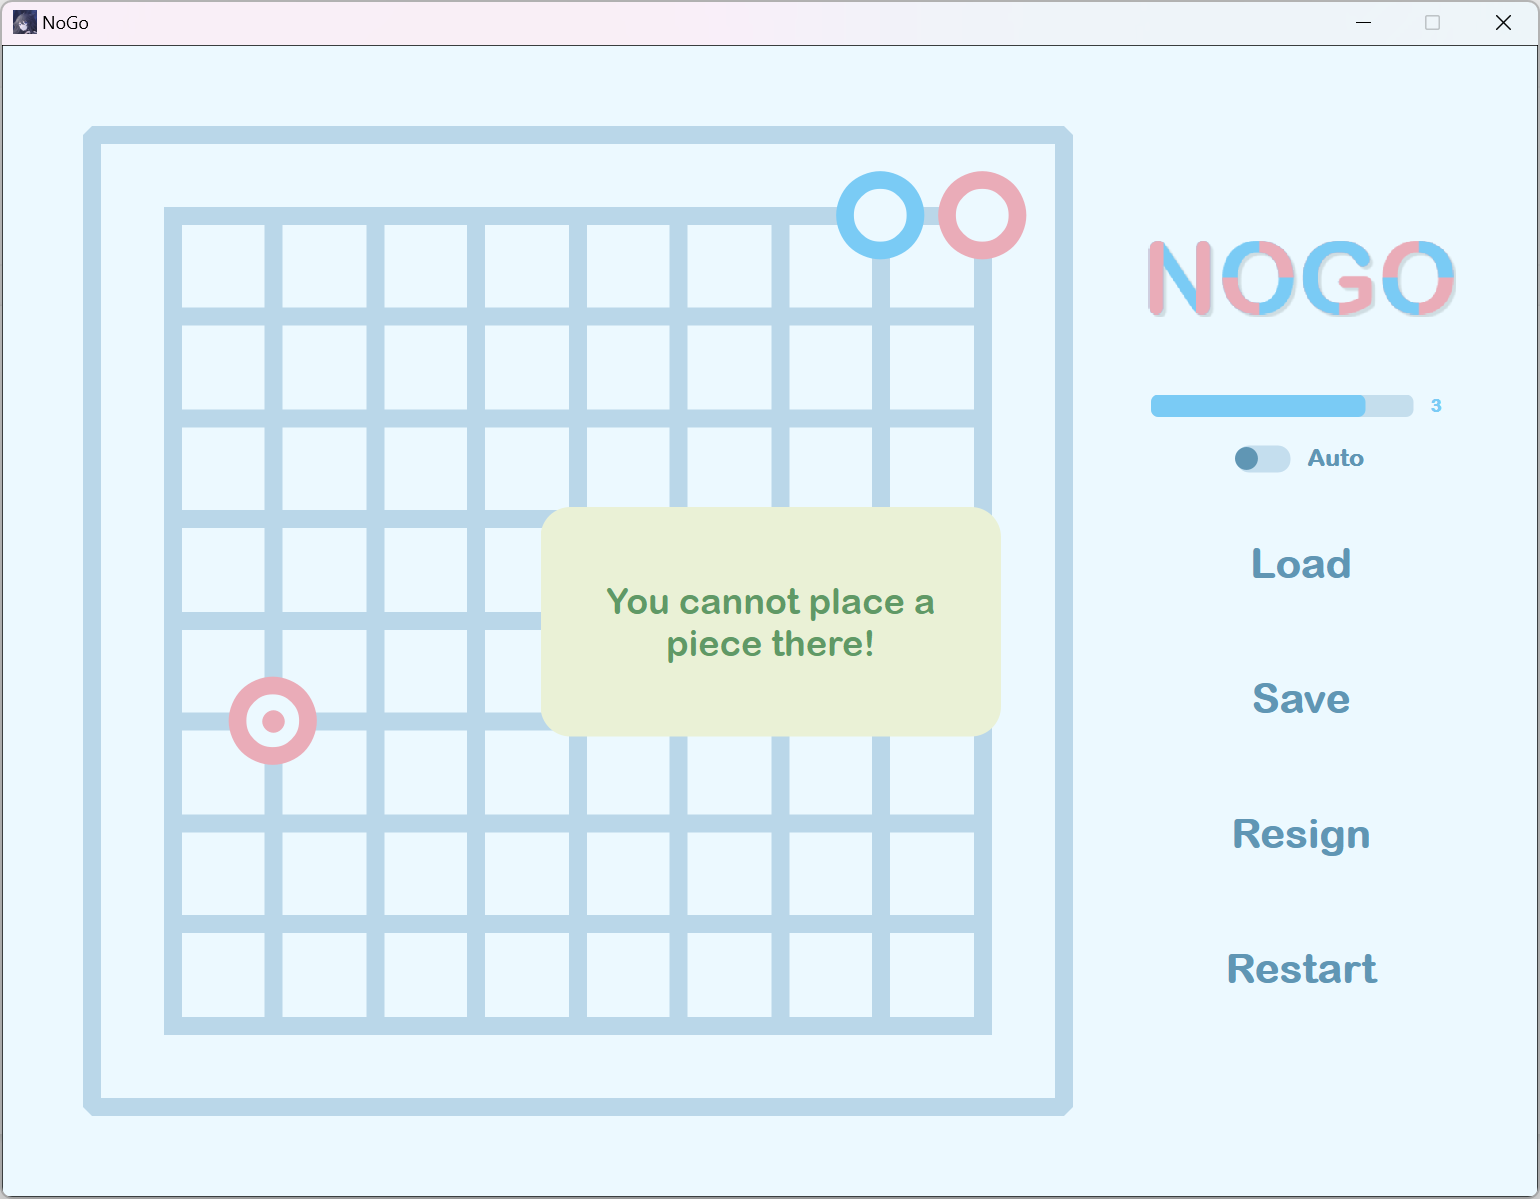
\includegraphics[width=5.5cm]{img/tip.png}
		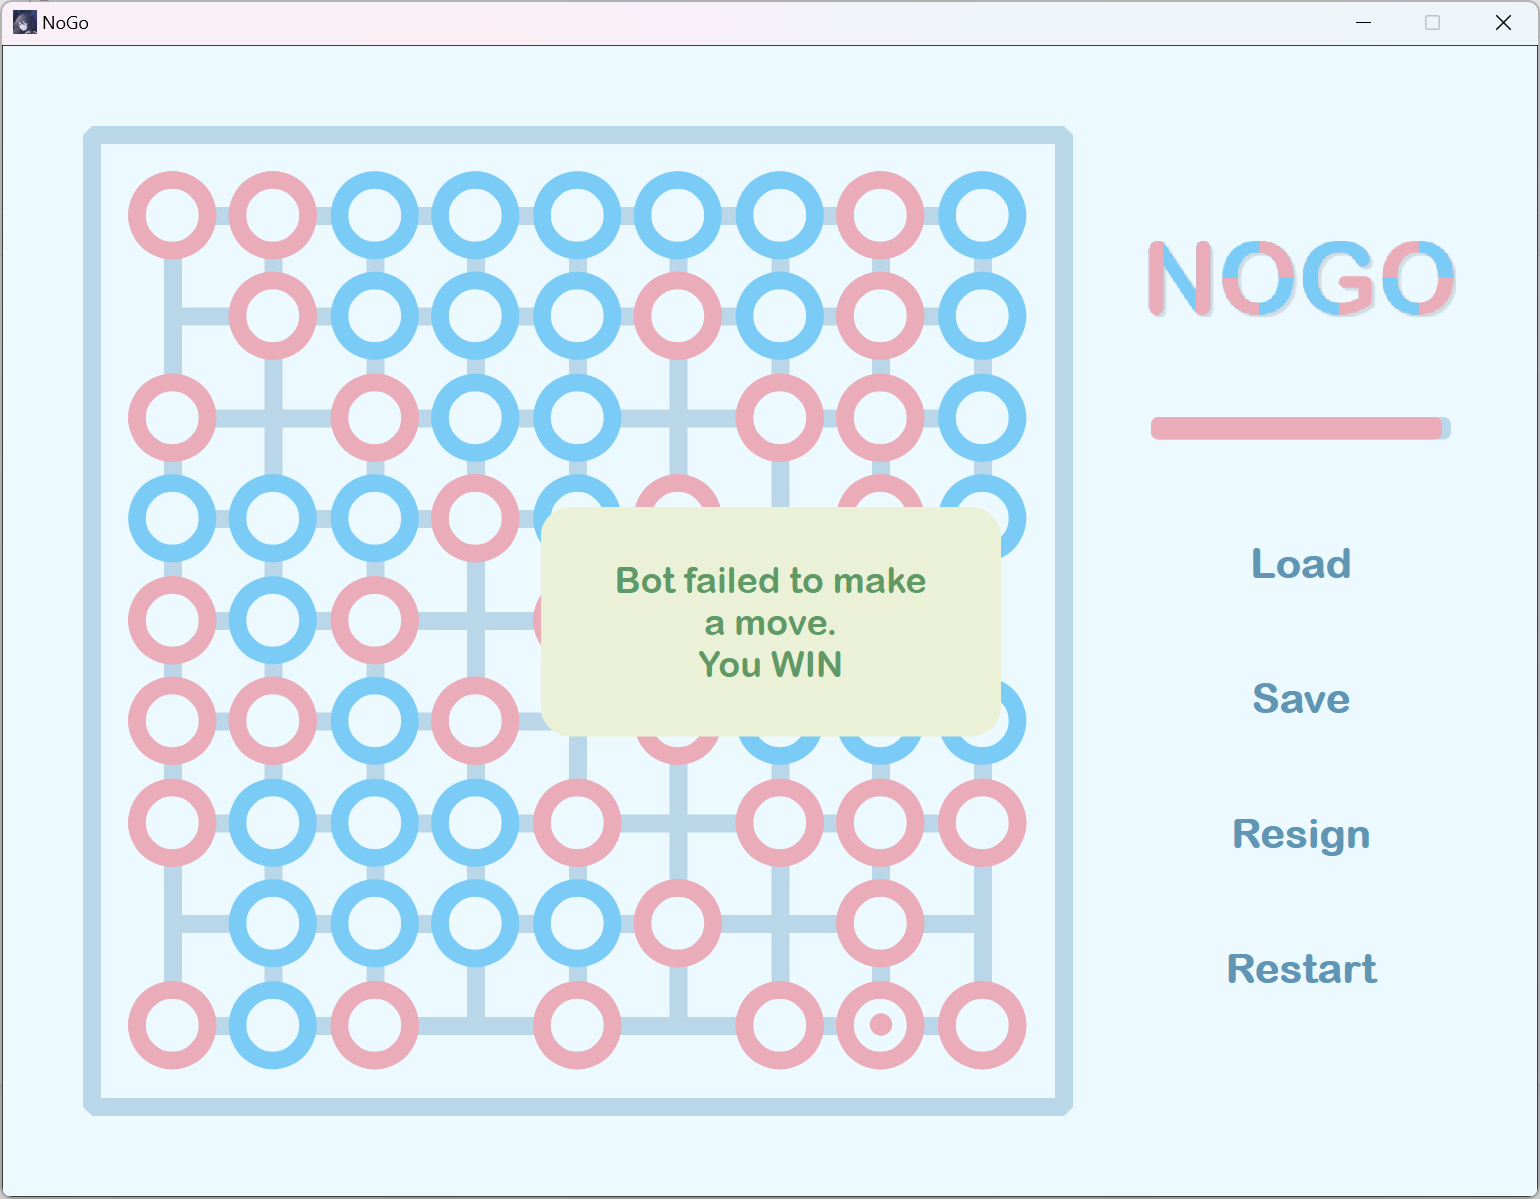
\includegraphics[width=5.5cm]{img/win.png}
		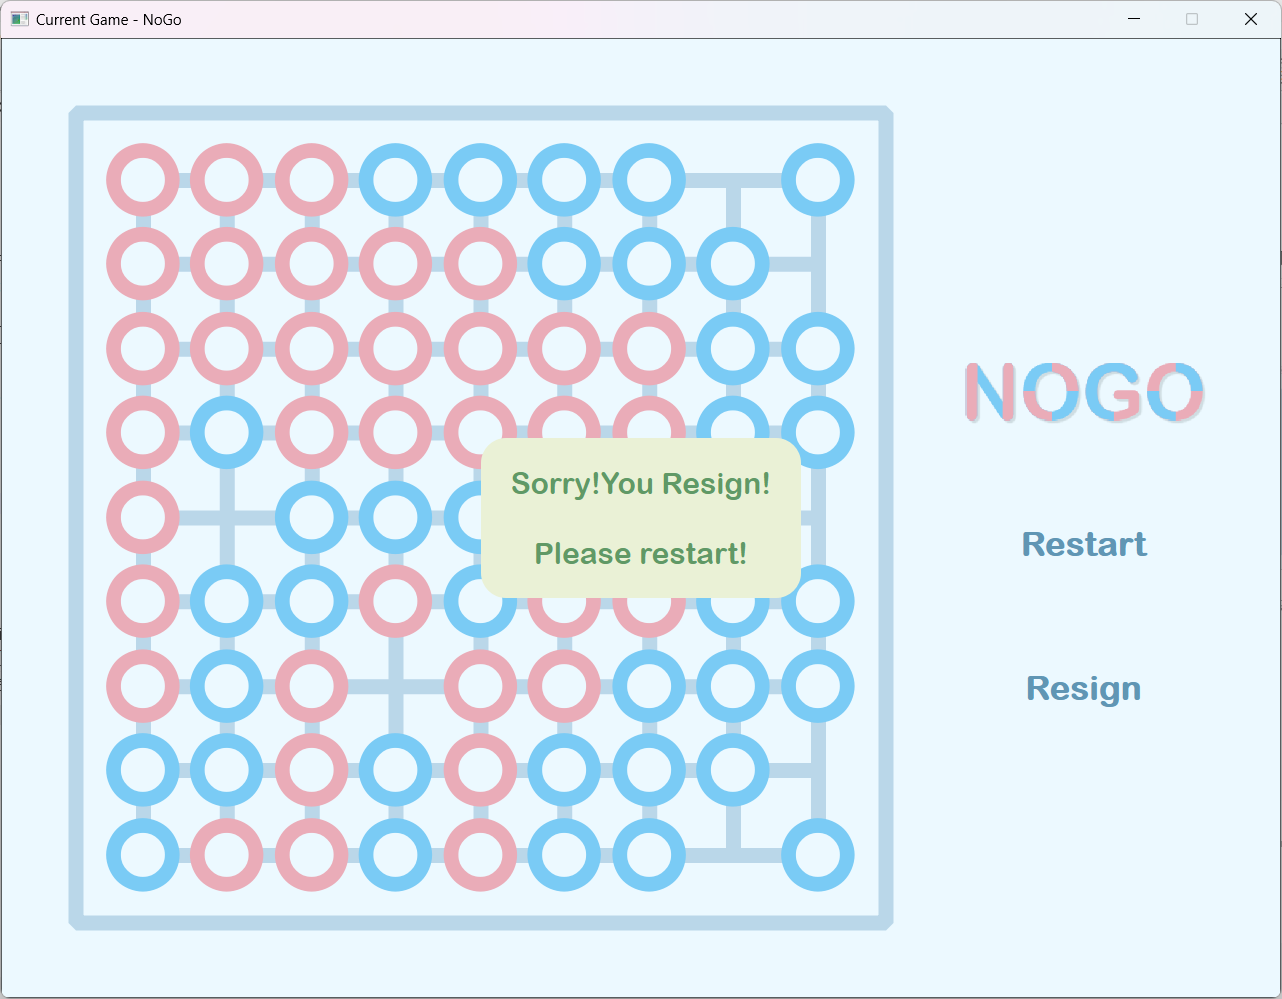
\includegraphics[width=5.5cm]{img/resign.png}
		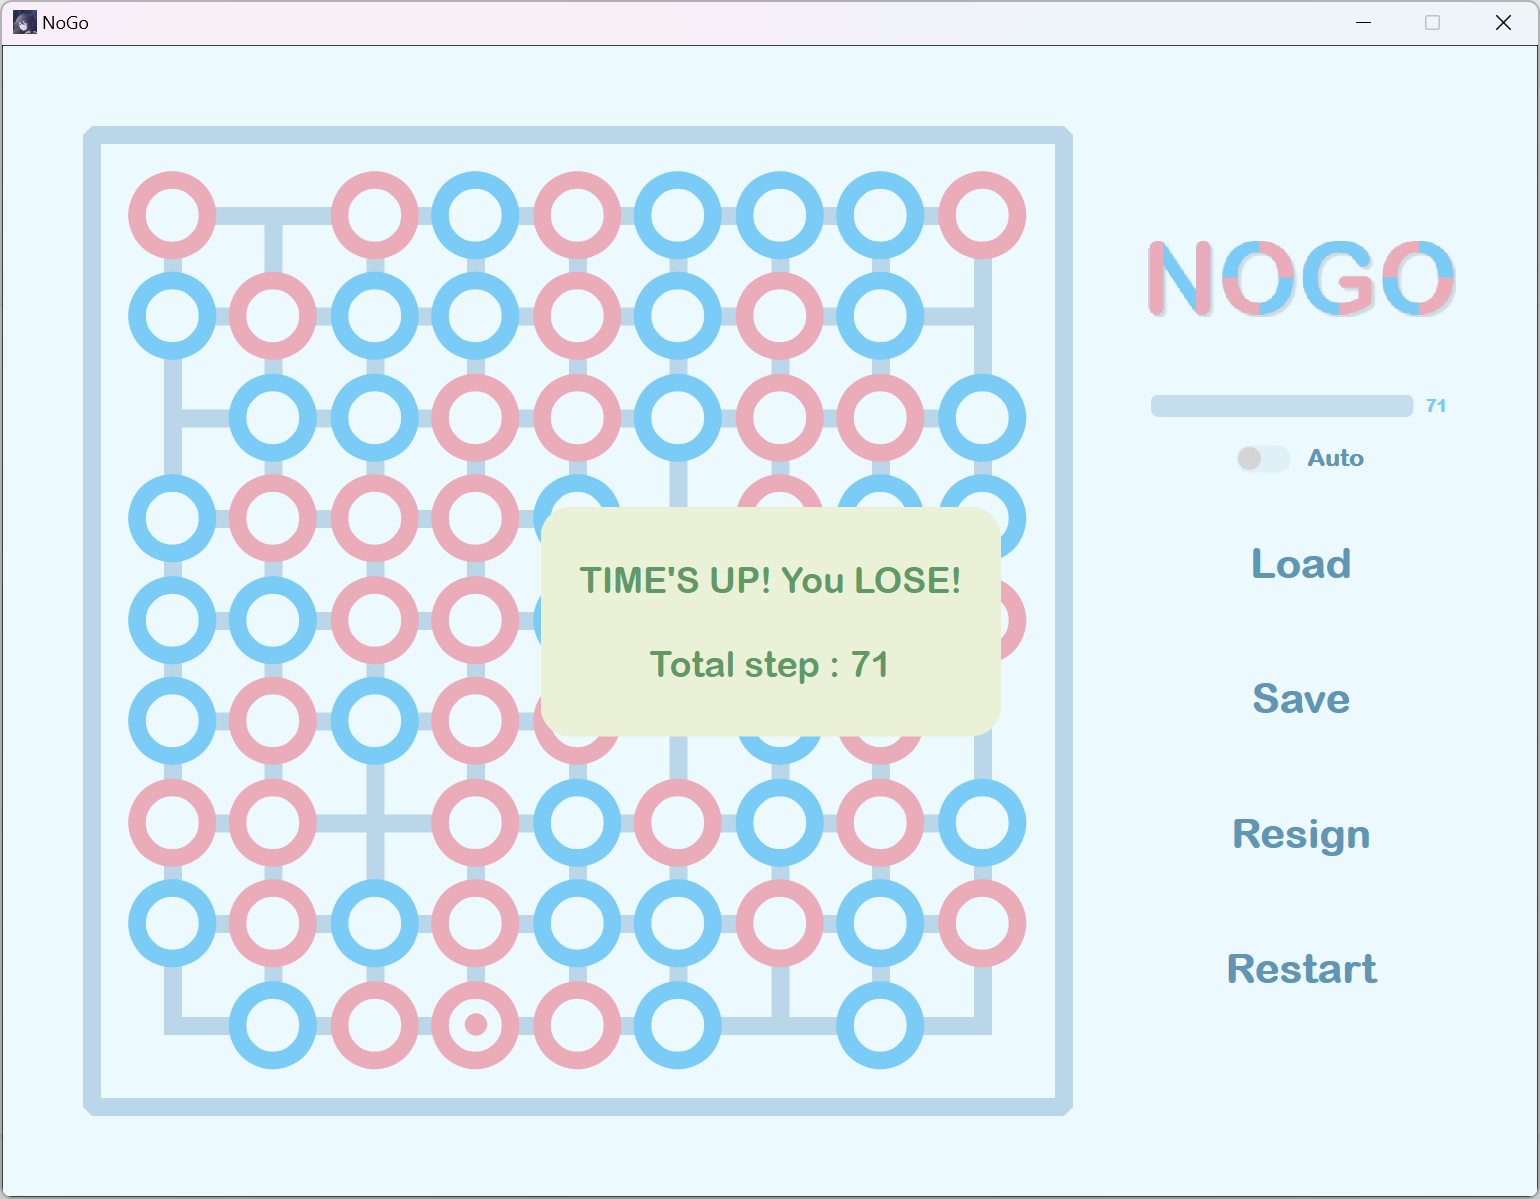
\includegraphics[width=5.5cm]{img/TLE.png}
		\counterwithin{figure}{subsection}
		\caption{状态判断}
	\end{figure}
	
	\subsection{设置}
	
	我们写了一个设置。
	
	\subsection{计时器}
	
	我们还没写好计时器。
	
	\subsection{更多功能}
	
	第一阶段还没结束,卷什么。
	
	在写了在写了。
	
	不如看一下隔壁队伍写的前后端分离。
	
	\section{AI 算法设计}
	
	由于现在还是第一阶段,所以我们采用了非常粗犷的 bot 写法:随机下棋。
	
	对于没有围棋基础的人来说,随机下棋的 bot 分布较好,bot 有获胜的可能。但是对于有基本围棋知识的人来说,只要斜着下棋、构造活眼就可以几乎 $100\%$ 战胜这个随机下棋 bot。
	
	\subsection{min-max 搜索和 $\alpha-\beta$ 剪枝}
	
	别卷了,还没写,你家程设就 $2$ 分。
	
	\section{感谢}
	
	感谢孙亚辉老师、潘俊达助教在学习生活上的指导和关心。
	
	感谢中国人民大学图灵实验班提供交流的平台与机会。
	
	感谢冯友和、赵培宇同学组成的团队。
	
	感谢彭文博、李知非同学于 2023/3/2 军理课后请本队吃的 KFC 疯狂星期四。
	
	感谢北京大学 ghastlcon 同学提供的帮助。
	
\end{document}